%%% PREAMBLE

\documentclass{article}
\usepackage{amsmath,amssymb,amsthm,fullpage,graphicx,subcaption}

% Use break between paragraphs instead of indentation
%\usepackage{parskip}

% Code highlighting
\usepackage[utf8]{inputenc}
\usepackage{listings, color}

% Default fixed font does not support bold face
\DeclareFixedFont{\ttb}{T1}{txtt}{bx}{n}{9} % for bold
\DeclareFixedFont{\ttm}{T1}{txtt}{m}{n}{9}  % for normal

% Custom colors
\usepackage{color}
\definecolor{deepblue}{rgb}{0,0,0.5}
\definecolor{deepred}{rgb}{0.6,0,0}
\definecolor{deepgreen}{rgb}{0,0.5,0}

% Python style for highlighting
\newcommand\pythonstyle{\lstset{
language=Python,
basicstyle=\ttm,
otherkeywords={self},             % Add keywords here
keywordstyle=\ttb\color{deepblue},
emph={MyClass,__init__},          % Custom highlighting
emphstyle=\ttb\color{deepred},    % Custom highlighting style
stringstyle=\color{deepgreen},
frame=tb,                         % Any extra options here
showstringspaces=false,           % 
commentstyle=\ttm\color{magenta}
}}

% Python environment
\lstnewenvironment{python}[1][]
{
\pythonstyle
\lstset{#1}
}
{}

% Python for external files
\newcommand\pythonex[2][]{{
\pythonstyle
\lstinputlisting[#1]{#2}}}

% Python for inline
\newcommand\pyln[1]{{\pythonstyle\lstinline!#1!}}

% Various math conveniences
\theoremstyle{definition}
\newtheorem*{prop}{Proposition}
\newtheorem*{obs}{Observation}
\newtheorem*{lemma}{Lemma}
\newtheorem*{disc}{Discussion}
\newtheorem*{qn}{Question}
\renewcommand{\bar}{\overline}
\newcommand{\nin}{\not\in}
\renewcommand{\>}{\rangle}
\newcommand{\<}{\langle}



%%% FILE INFO

% Header
%\usepackage{fancyhdr}
%\usepackage[margin=1in, headheight=50pt]{geometry}
%\pagestyle{fancy}
%\lhead{\textbf{CS21}}
%\chead{Final}
%\rhead{Aritra Biswas}
%\setlength{\headsep}{20pt}

% Title stuff
\title{\textbf{Set 1: Lissajous Figures and Beats}}
\date{}
\author{Aritra Biswas}



%%% DOCUMENT

\begin{document}

\maketitle

\section{Computing sinusoids}

We compute sequences of the following trigonometric functions:
\begin{align}
X(t) &= A_X \cos(2\pi f_X t) \\
Y(t) &= A_Y \sin(2\pi f_Y t + \phi) \\
Z(t) &= X(t) + Y(t)
\end{align}

for $t=n\Delta t$ with $n=0,\dots,N$. We do this first with
\pyln{python} lists:

\pythonex{computeXYZ_python.py}

The program can be made neater and more efficient with
\pyln{numpy} arrays. We rewrite the following two functions:

\pythonex[firstline=10, lastline=23]{computeXYZ_numpy.py}

To save the data to an ASCII file as desired, we can redirect
output to a file at runtime, or in the \pyln{numpy} version we can
simply replace \pyln{sys.stdout} with the desired file.

\section{Lissajous figures}

We generate Lissajous figures as follows, using
\pyln{varf} and \pyln{varphi} as necessary in the interpreter. Predetermined
conditions are: $A_X = 1, A_Y = 2, \phi = 0.5, dt = 0.001, N = 1000)$.

\pythonex{lissajous.py}

\subsection{Closed curves when $f_X/f_Y$ is rational}

\begin{prop}
If $f_X/f_Y$ is a rational number, then the Lissajous figure is a closed curve.
\end{prop}

\begin{proof}
A sinusoidal function $\sin(\omega t)$ has period $2\pi / \omega$. Thus
$X(t)$ has period $1/f_X$ and $Y(t)$ has period $1/f_Y$. In other
words, for all integers $j$ and $k$, we have:
\begin{align*}
X(t + j/f_X) = X(t)\text{ and }Y(t + k/f_Y) = Y(t)
\end{align*}
Since $f_X/f_Y$ is rational, it can be written as a fraction of two integers.
Let $f_X/f_Y = j/k$ where $j$ and $k$ are integers. Then $j/f_X = k/f_Y$.
Let $\varphi = j/f_X = k/f_Y$. Then, for any point,
$X(t+\varphi) = X(t)$ and $Y(t+\varphi) = Y(t)$.

Thus, for any point $(X(t),Y(t))$, there exists an identical point
$(X(t+\varphi),Y(t+\varphi))$ in the parametrization,
so each point is revisited infinitely many times, implying
the graph is a closed curve.
\end{proof}

\begin{figure}\centering
\begin{subfigure}{0.48\textwidth}\centering
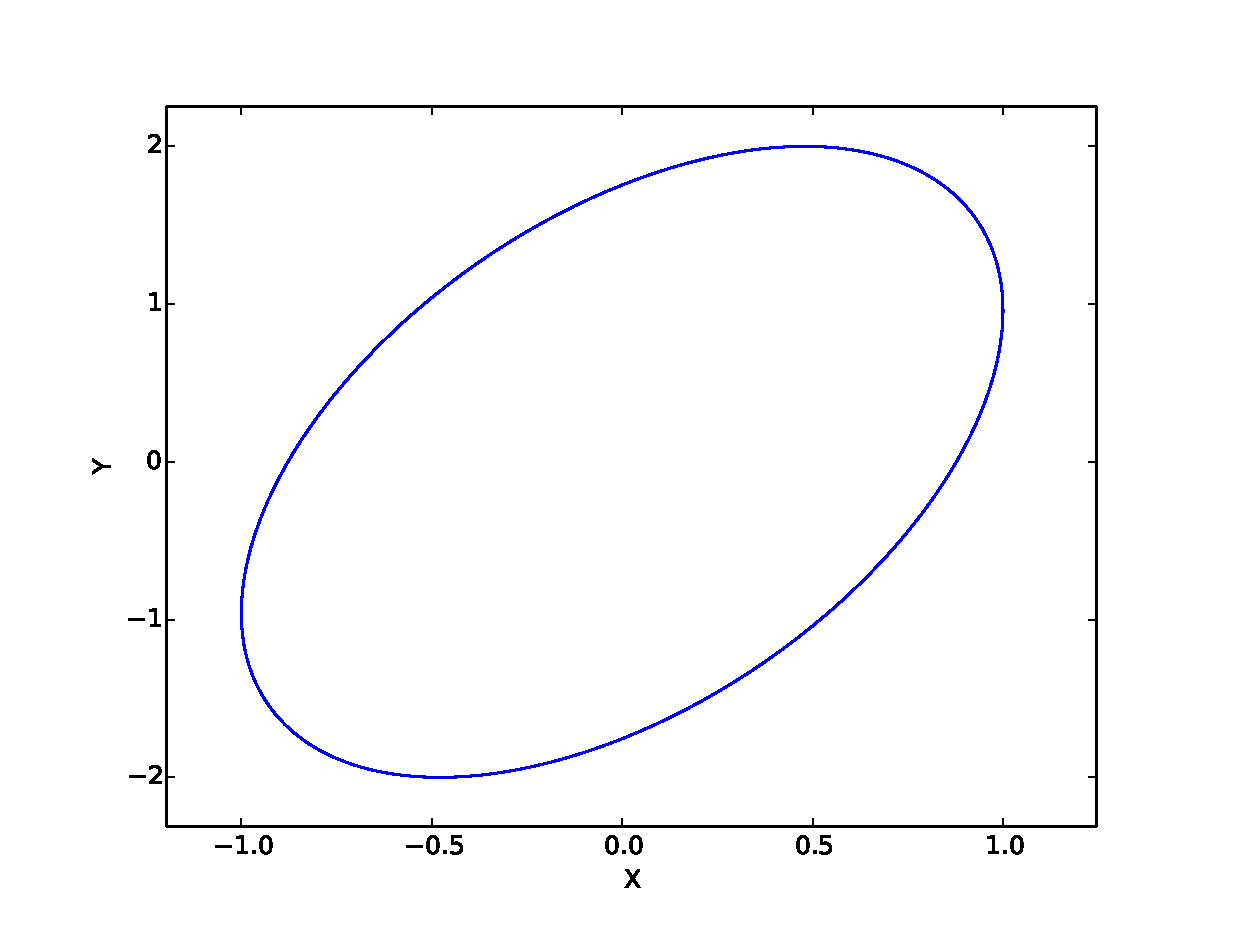
\includegraphics[width=\textwidth]{figure_1.eps}
\caption{$f_X/f_Y = 1$}
\end{subfigure}
\begin{subfigure}{0.48\textwidth}\centering
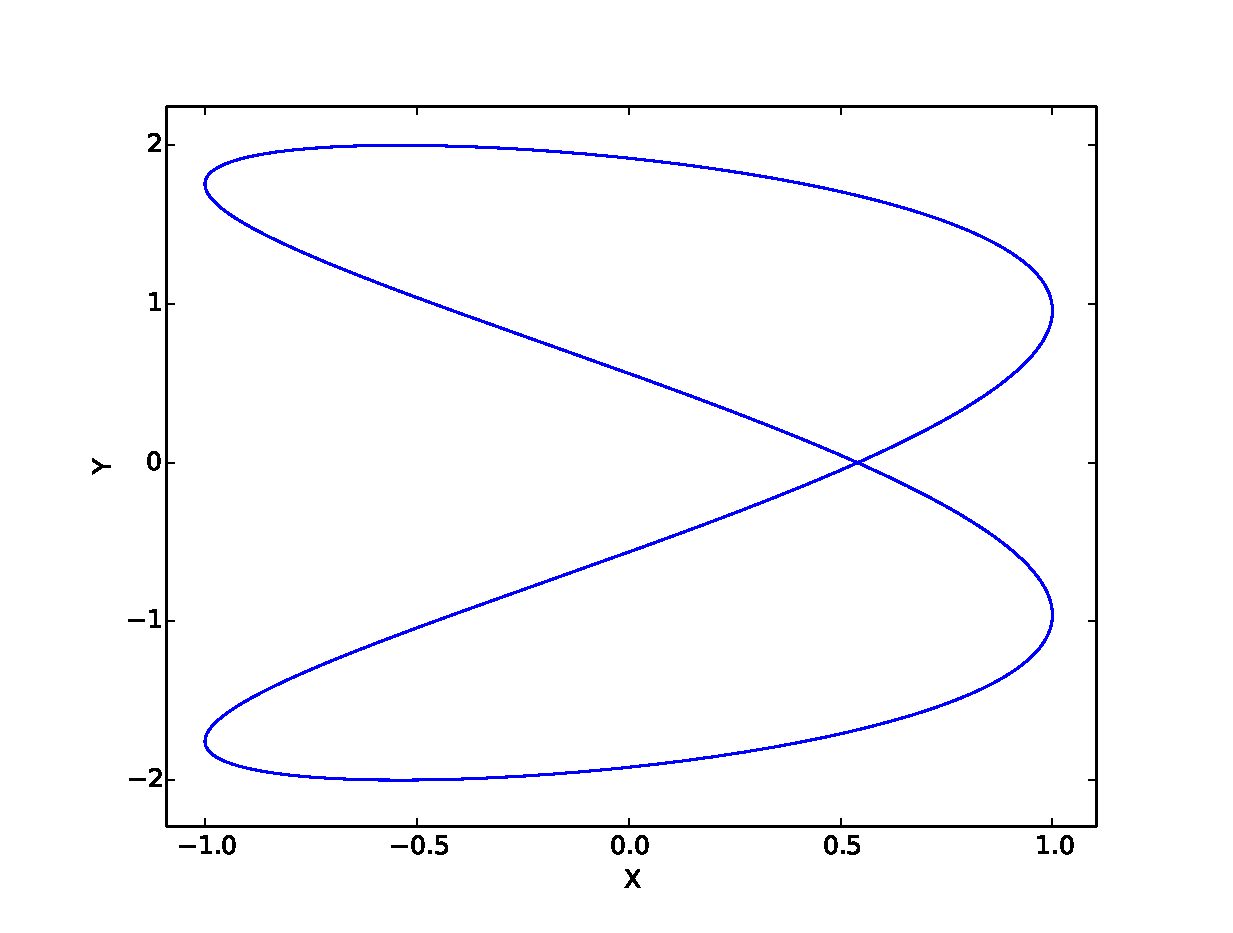
\includegraphics[width=\textwidth]{figure_2.eps}
\caption{$f_X/f_Y = 2$}\label{fig:flip}
\end{subfigure}
\begin{subfigure}{0.48\textwidth}\centering
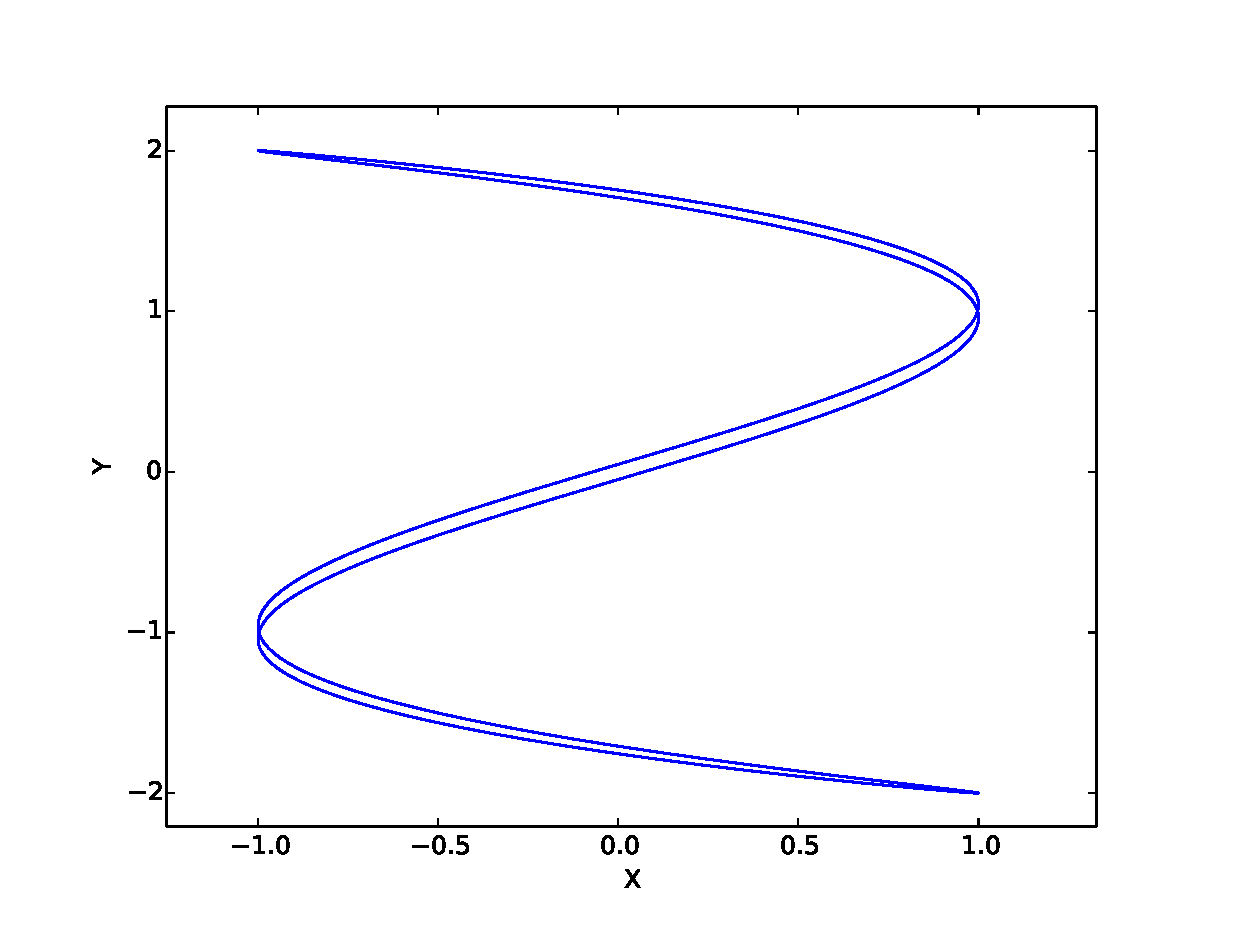
\includegraphics[width=\textwidth]{ratio3.eps}
\caption{$f_X/f_Y = 3$}
\end{subfigure}
\begin{subfigure}{0.48\textwidth}\centering
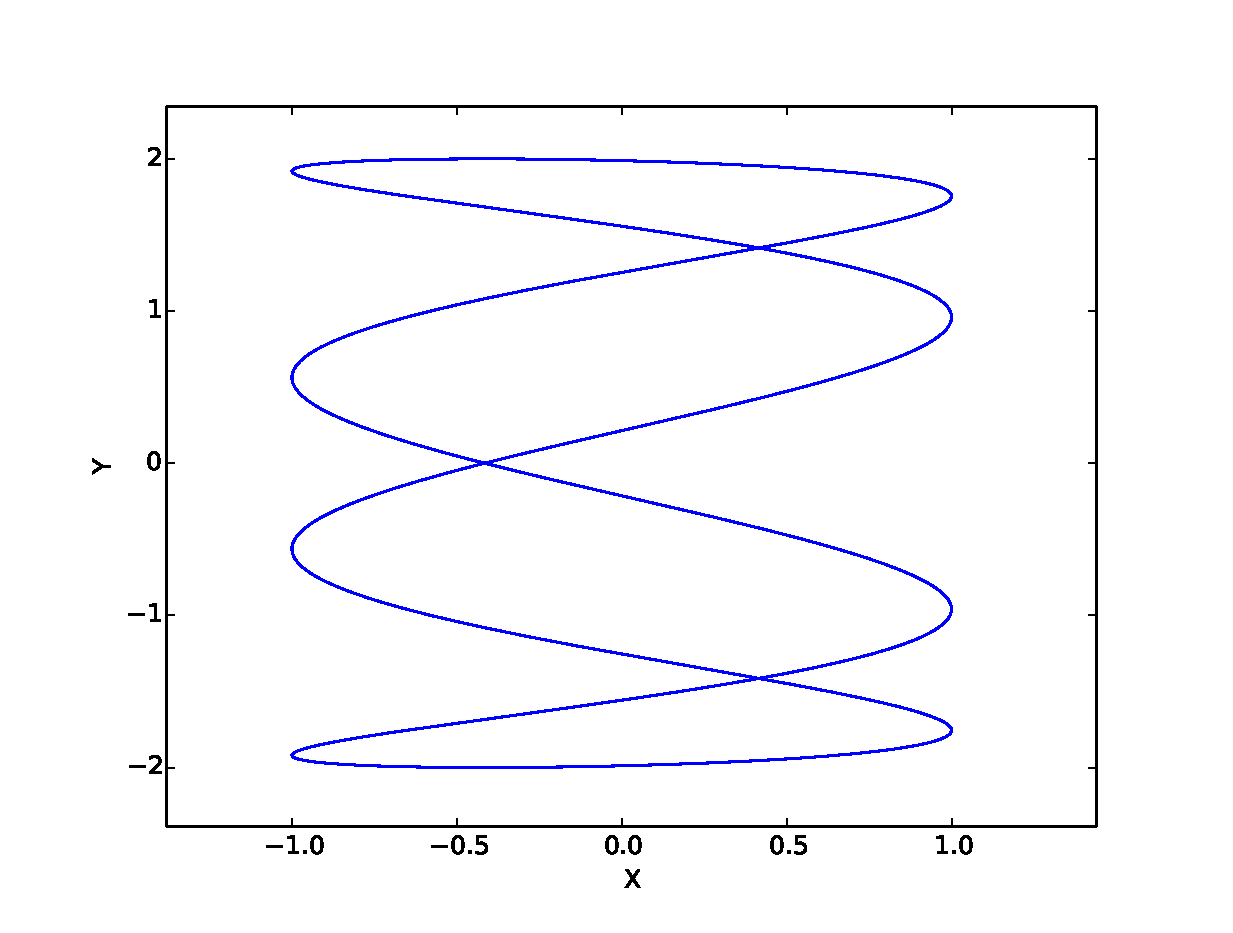
\includegraphics[width=\textwidth]{ratio4.eps}
\caption{$f_X/f_Y = 4$}
\end{subfigure}
\begin{subfigure}{0.48\textwidth}\centering
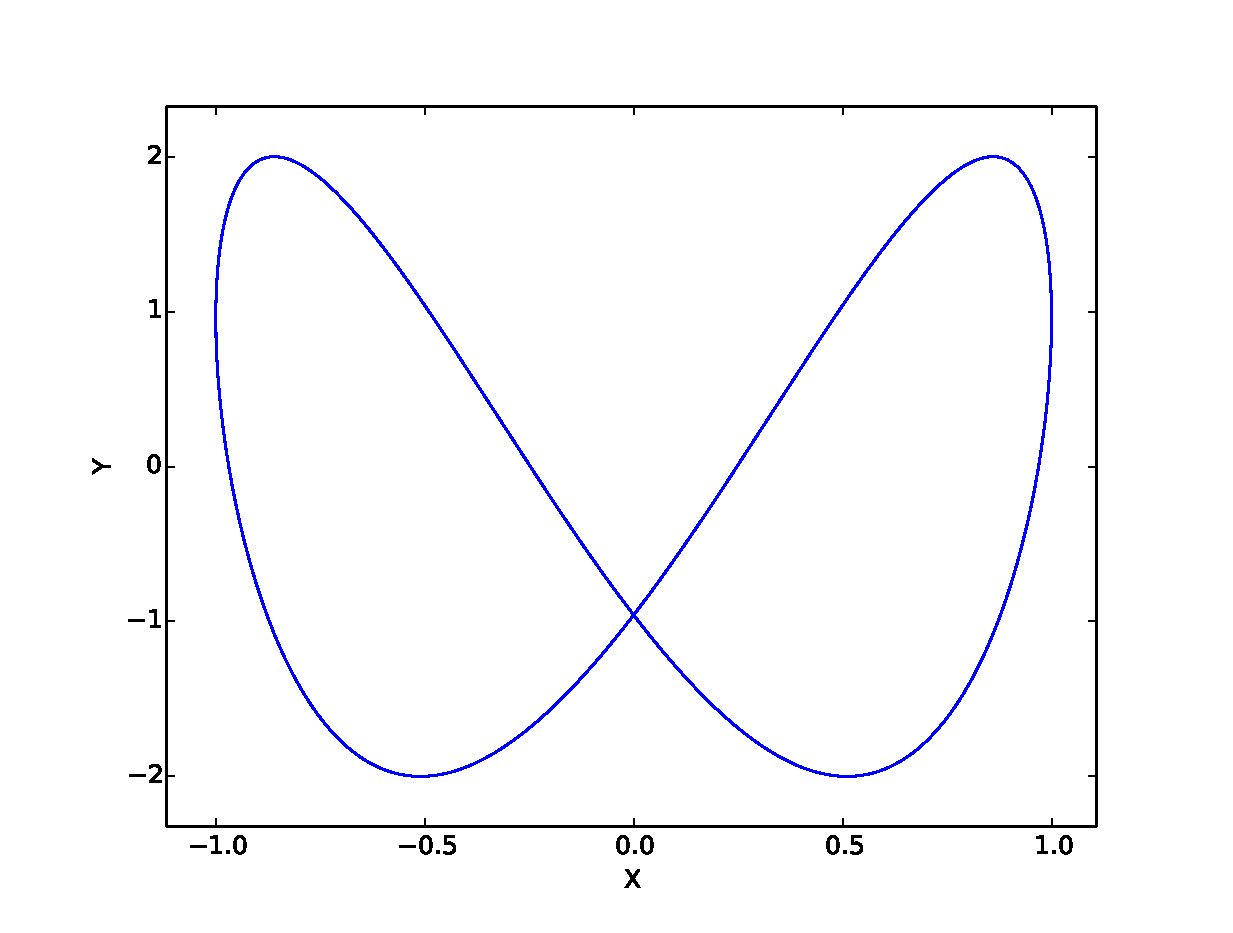
\includegraphics[width=\textwidth]{figure_3.eps}
\caption{$f_X/f_Y = 1/2$}\label{fig:oflip}
\end{subfigure}
\begin{subfigure}{0.48\textwidth}\centering
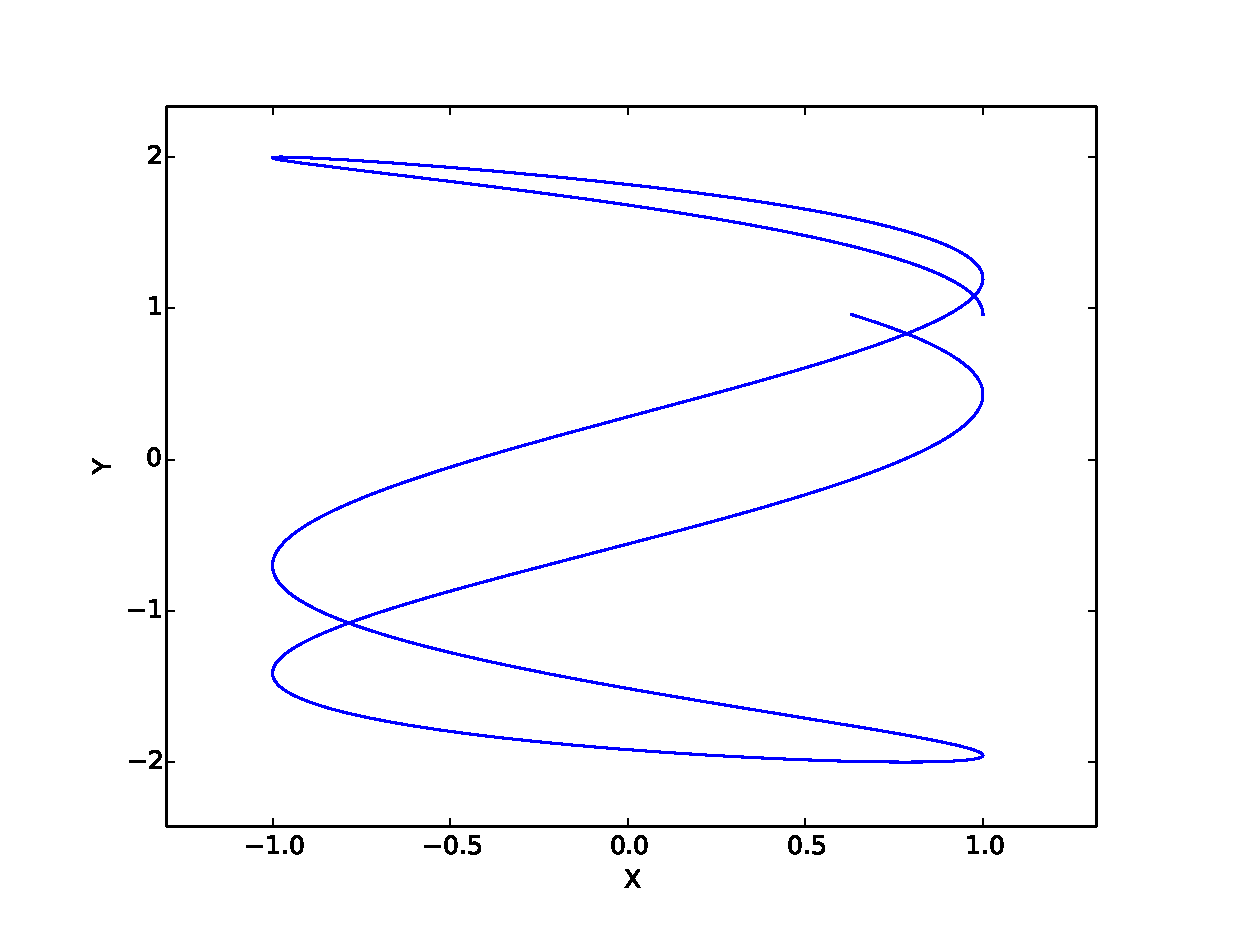
\includegraphics[width=\textwidth]{figure_4.eps}
\caption{$f_X/f_Y = \pi$}\label{fig:spec}
\end{subfigure}
\caption{Lissajous figures with various $f_X/f_Y$.}\label{fig:varfrat}
\end{figure}

Figure \ref{fig:varfrat} illustrates this phenomenon. Notably, the curve in
\ref{fig:spec} would actually be closed if we plotted with high enough $N$,
since the program uses \pyln{np.pi}, a finite-length rational approximation
of $\pi$.

\subsection{Effect of $f_X/f_Y$ on curve shape}

From Figure \ref{fig:varfrat}, we can infer some apparent patterns. The
relationship between figures \ref{fig:flip} and \ref{fig:oflip} suggests that
inverting $f_X/f_Y$ causes the Lissajous figure to flip over the $Y=-X$ line.

Furthermore, when $f_X > f_Y$, increasing the ratio seems to increase the
number of turns in the loop. Given the prior observation, this suggests
that the opposite will be true when $f_Y > f_X$.

We also consider the special case with $f_X=2$, $f_Y=1$, and $\phi=0$,
shown in figure \ref{fig:special}. Although the figure doesn't enclose an area,
it is closed in the sense that every point is revisited infinitely many times
in a parametrization of the curve. In the time that $Y(t)$ completes a cycle
(-1 to 1 and back to -1), $X(t)$ completes two (-1 to 1 -1 on the way up,
and another cycle on the way down).

\begin{figure}\centering
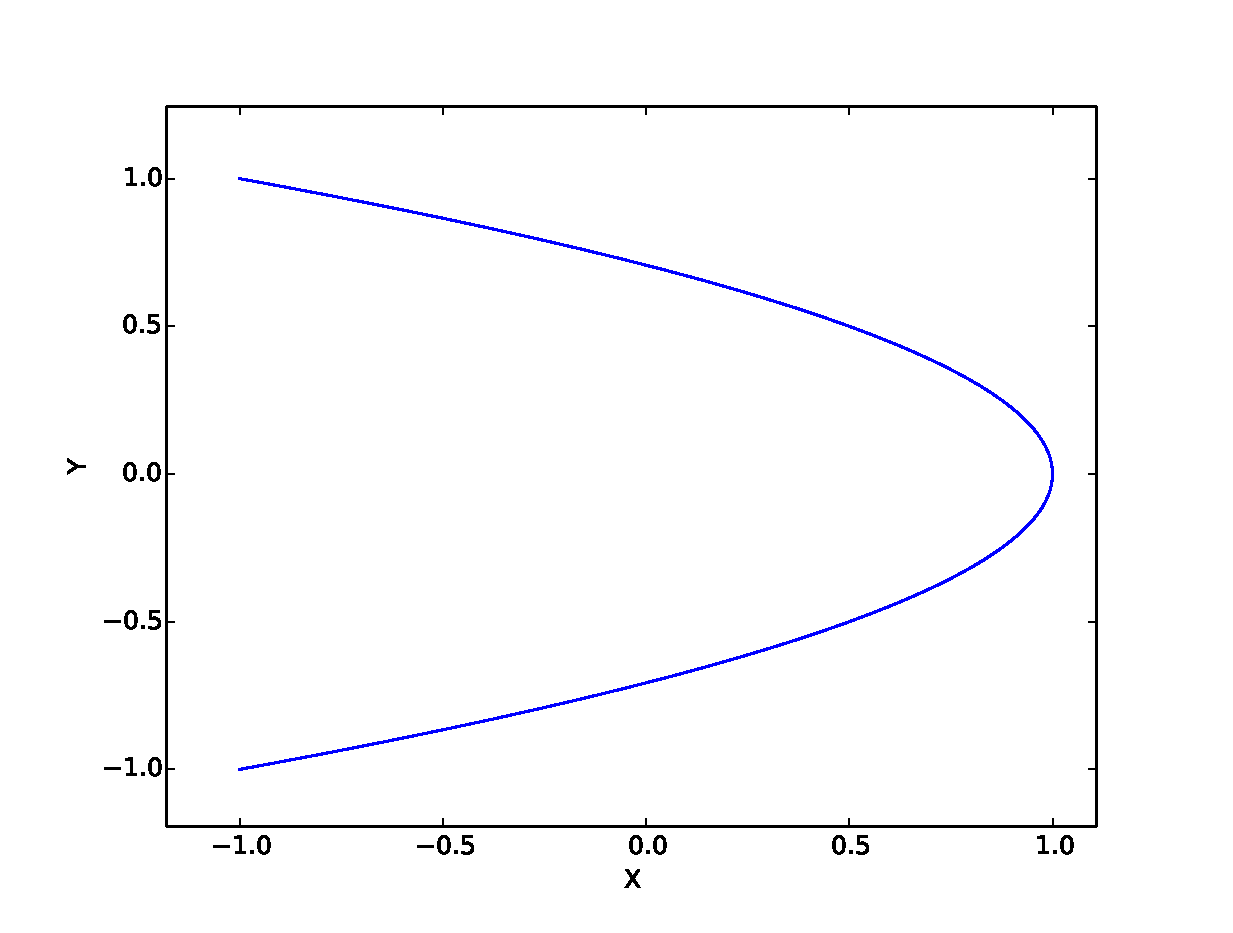
\includegraphics[width=0.9\textwidth]{special.eps}
\caption{Lissajous figure with $f_X=2$, $f_Y=1$, and $\phi=0$.}\label{fig:special}
\end{figure}

\subsection{Effect of phase shift $\phi$ with $f_X=f_Y$}

Whenever $\phi$ is an integer multiple of $\pi$, the Lissajous figure is
circular (identical to the red curve with $\phi=0$ in figure \ref{fig:varphi}).

\begin{figure}\centering
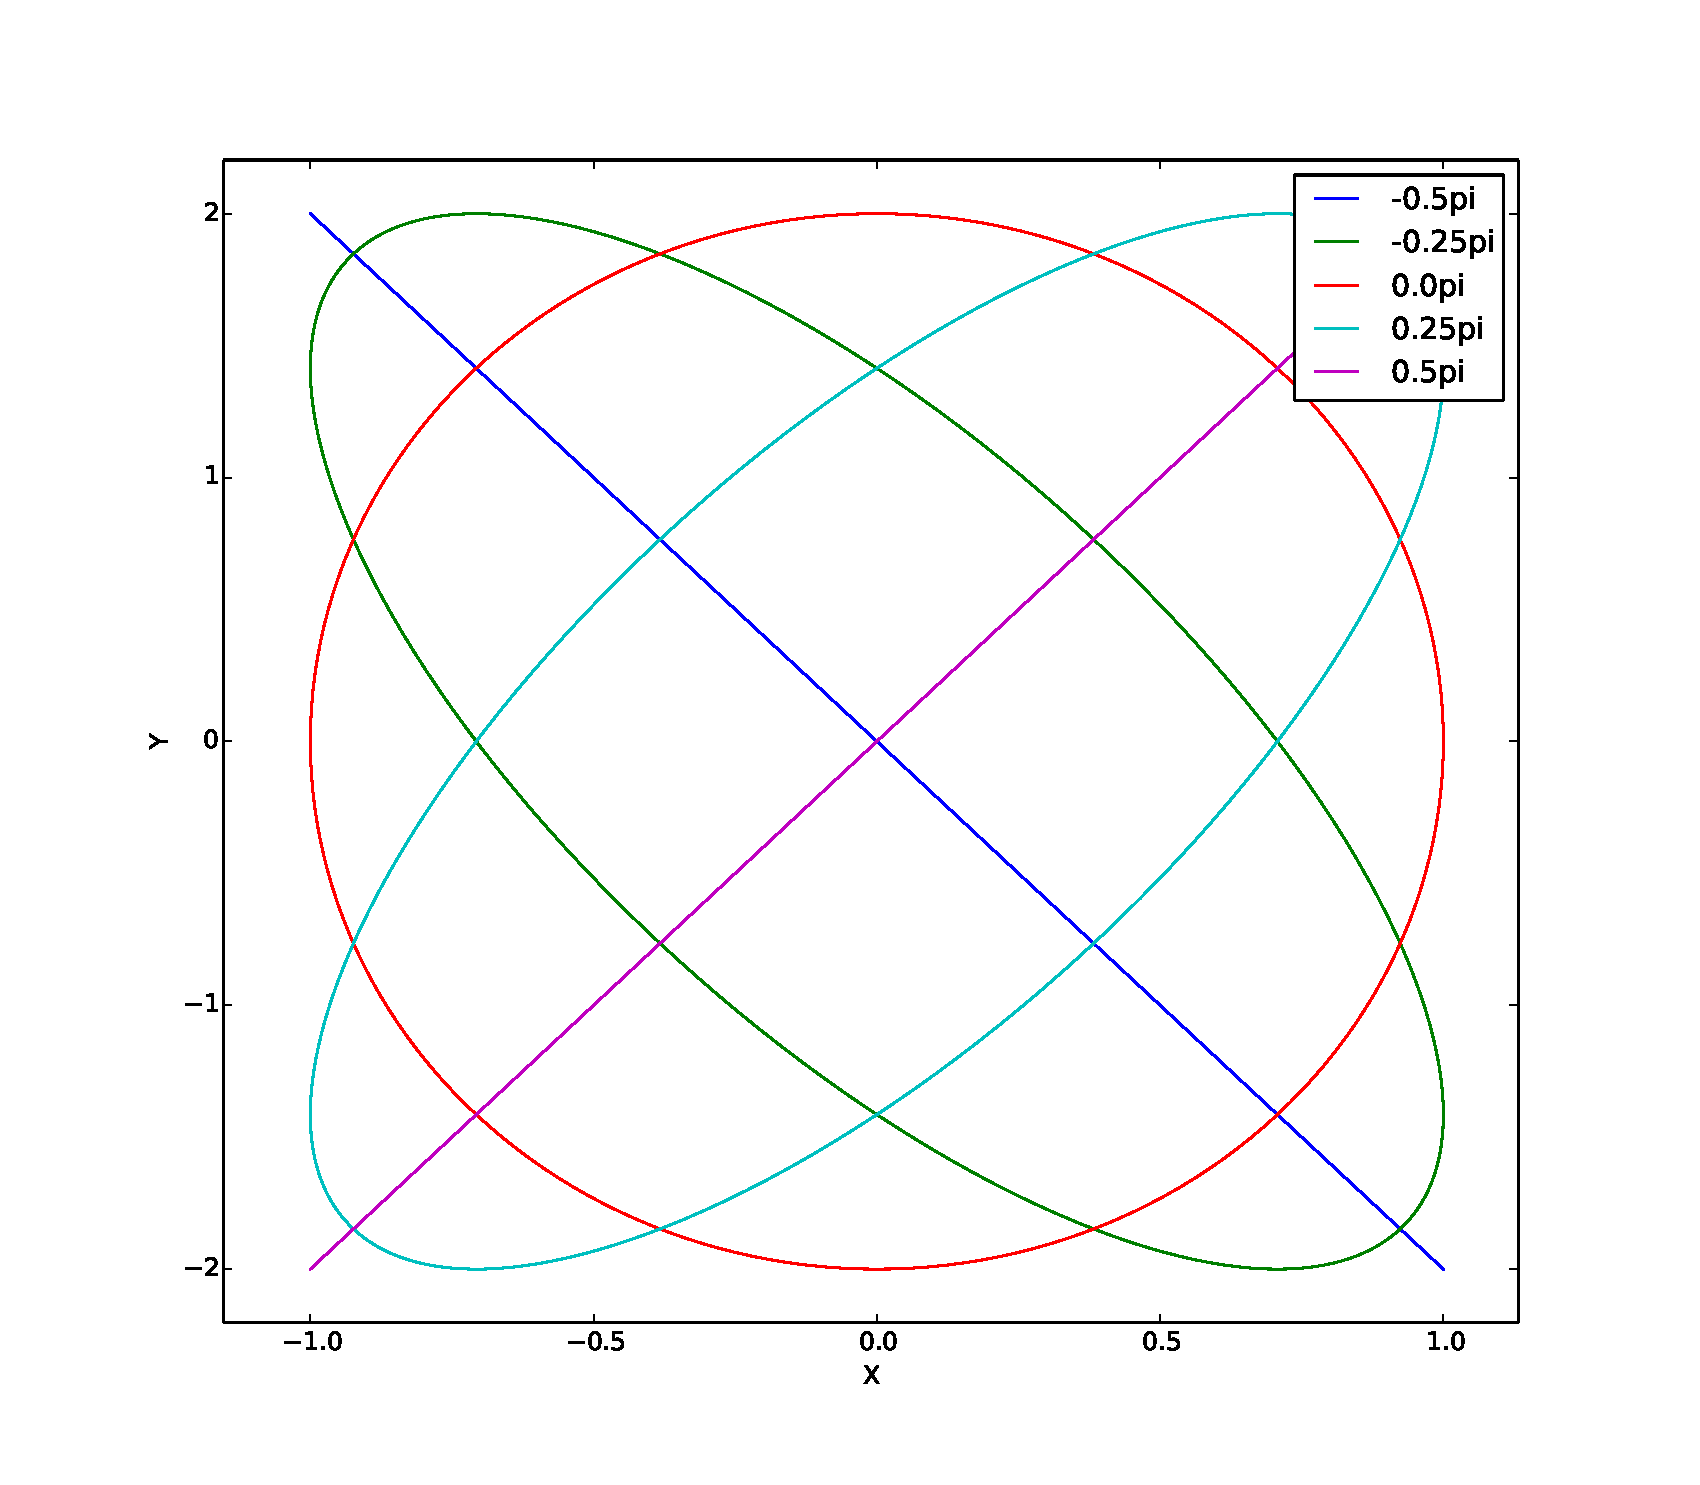
\includegraphics[width=0.9\textwidth]{varphi.eps}
\caption{Lissajous figures with varying $\phi$ values.}\label{fig:varphi}
\end{figure}

Furthermore, figure \ref{fig:varphi} also shows that the Lissajous figure
deviates from a circular shape as $\phi$ becomes farther from an integer
multiple of $\pi$.

Thus, the Lissajous figure shows
how close two sinusoids are to being exactly in or out of phase. To tune
circuits using an
oscilloscope, one can adjust the phase shift until the visible Lissajous
figure is circular.

\section{Beats}

We generate the $Z(t)$ vs. $t$ graph, and optionally its Fourier transform,
in \pyln{plotZ}, with the predetermined conditions $A_X = 1, A_Y = 1, \phi = 0.5, dt = 0.001,
N = 50000$.

\pythonex{beats.py}

We use $f_X=1.1$ and $f_Y=1$.
The periods corresponding to $\omega_1$ and $\omega_2$ are
given by:

\begin{align*}
T\left(\frac{\omega_1 + \omega_2}{2}\right) &= \frac{4\pi}{2\pi f_X + 2\pi f_Y}
= \frac{2}{f_X + f_Y} = \frac{2}{1.1 + 1} = 0.952381 \\
T(\omega_1 - \omega_2) &= \frac{2\pi}{2\pi f_X - 2\pi f_Y}
= \frac{1}{0.1} = 10 \\
\end{align*}

Figure \ref{fig:Z} demonstrates many cycles with period 0.952381,
and modulation cycles with period 10.

As expected,
figure \ref{fig:Zh} exhibits a peak at each of the
component frequencies, $f_X = 1.1$ and $f_Y=1$.

\subsection{Symmetry as an explanation of modulation frequency doubling}

We explore why the modulation frequency is twice what is expected. In a generic case,
suppose we have two sinusoids $\cos(\omega_1 t)$ and $\cos(\omega_2 t)$. We know that
the sum of these two sinusoids is given by:
$$\cos(\omega_1 t) + \cos(\omega_2 t) = 2\cos\left(\frac{\omega_1 + \omega_2}{2}t\right)
\cos\left(\frac{\omega_1 - \omega_2}{2}t\right).$$

We can interpret this as a single sinusoid $Z(t) = A\cos\left(\frac{\omega_1 + \omega_2}{2}t\right)$,
with the changing amplitude given by $A(t) = 2\cos\left(\frac{\omega_1 - \omega_2}{2}t\right)$.
Since the amplitude is expressed as a $\cos$ function, the amplitude oscillates around 0, i.e.
$A<0$ half the time. ``Negative amplitude'' doesn't intuitively mean much to us; we can interpret
this as simply flipping the sinusoid $Z(t)$ about the $x$-axis when the amplitude is negative.
However, this is not visible because $\cos\left(\frac{\omega_1 + \omega_2}{2}t\right)$ is itself a
symmetric sinusoid, and flipping the curve about the $x$-axis twice
results in the original curve.

Thus, we can say that the amplitude
is given by $A(t) = \left| 2\cos\left(\frac{\omega_1 - \omega_2}{2}t\right) \right|$, which has half
the period (i.e. twice the frequency), so the amplitude modulation frequency is simply $\omega_1 - \omega_2$.

\begin{figure}\centering
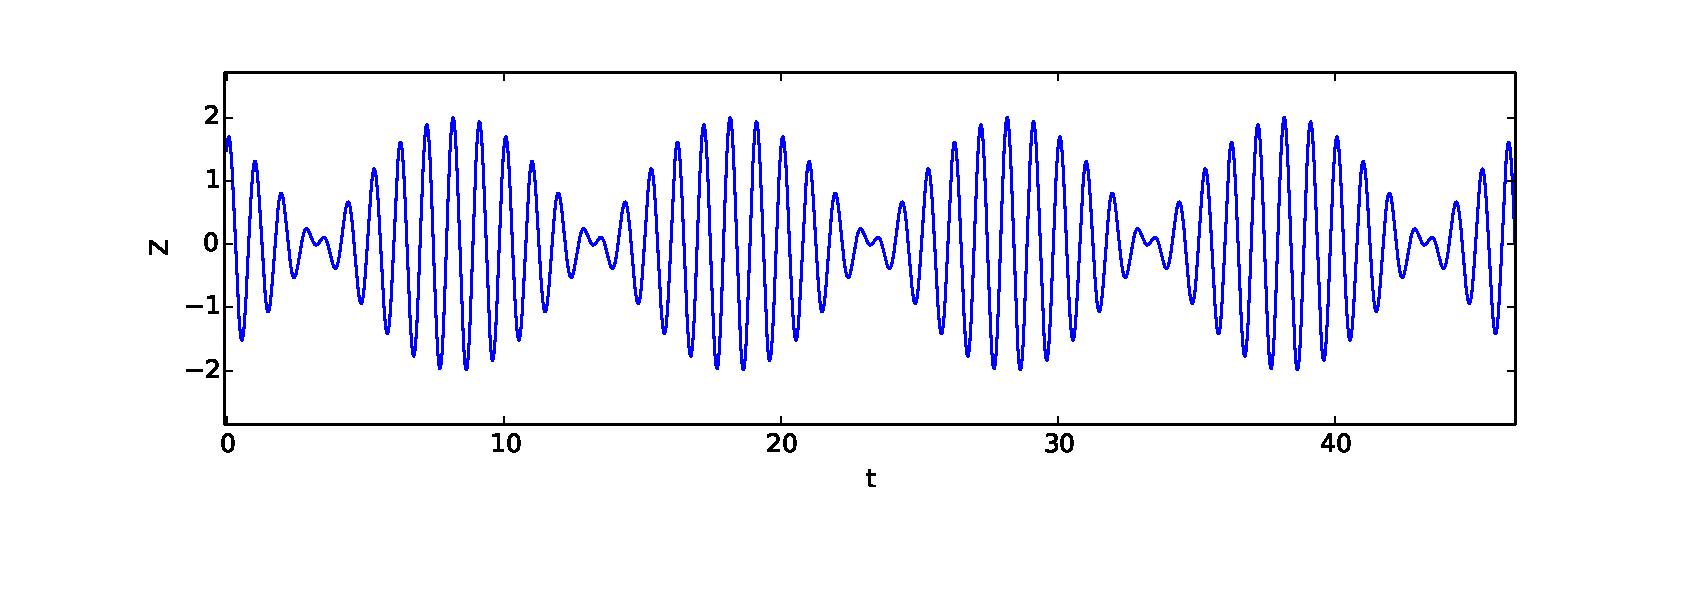
\includegraphics[width=\textwidth]{Z.eps}
\caption{$Z(t)$ vs. $t$, with $f_X = 1.1$ and $f_Y = 1$.}\label{fig:Z}
\end{figure}

\begin{figure}\centering
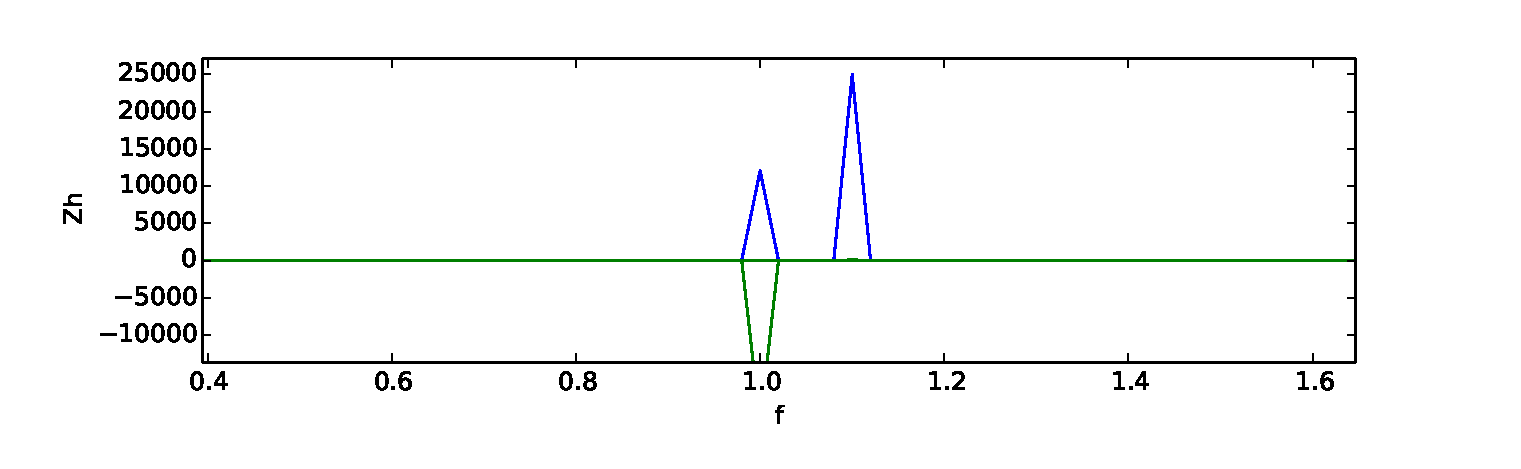
\includegraphics[width=\textwidth]{Zh.eps}
\caption{$\hat Z(f)$ vs. $f$, showing component frequencies $f_X = 1.1$ and $f_Y = 1$.}\label{fig:Zh}
\end{figure}

\section{Programming Reflections}

I've programmed in C and Python before. Python is more high-level, so it's a lot
more convenient for numerical applications such as these. Guido van Rossum's
description of Python touts its ``efficient high-level data structures,''
``elegant syntax and dynamic typing,'' features which make Python code
simpler and shorter. However, Python is notably inefficient. For example,
Python 2's \pyln{range} function returns an actual list, so using it
to loop through the indices of a string (e.g. \pyln{for i in range(len(string))})
requires storing the entire list in memory. In C, we can
just store a counter variable: \pyln{for (i = 0, i < strlen(string), i++)}.

\pyln{numpy} has the added advantage of data structures designed specifically
for numerical analysis. Since we deal with operations on arrays so often,
it's very convenient to be able to operate on elements of a \pyln{np.array}
object by treating the array name as a variable,
while looping through the elements of the array is done
behind-the-scenes and efficiently with C.

\end{document}
